\section{Simulation}
In order to study the performance of the CND, its geometry and response were included in the CLAS12 Geant4-based simulation package, GEMC \cite{sim-nim}. The Birks effect, for which the number of optical photons produced for a given certain energy deposition in the scintillator depends on the particle type, and the hit digitization for the CND, have been introduced in GEMC.
The timing resolution and the energy loss due to the U-turn geometry were included in the simulation using the values measured in the cosmic-ray tests.
Details on the digitization and on the hit and event reconstruction are explained in \cite{sim-nim} and in \cite{recon-nim}, respectively.

Simulations were run to evaluate the efficiency of the CND for neutrons, its ability to discriminate between neutrons and photons, and its angular and momentum resolutions. Neutrons and photons of momenta varying between 0.1 and 1~GeV and having polar angles $\theta$ between $50^o$ and $70^o$ were generated at a fixed azimuthal angle ($\phi = 3.75^o$). Several values of energy thresholds, between 1 and 5 MeV, were studied.
\begin{figure}[htb]  
\begin{center}
%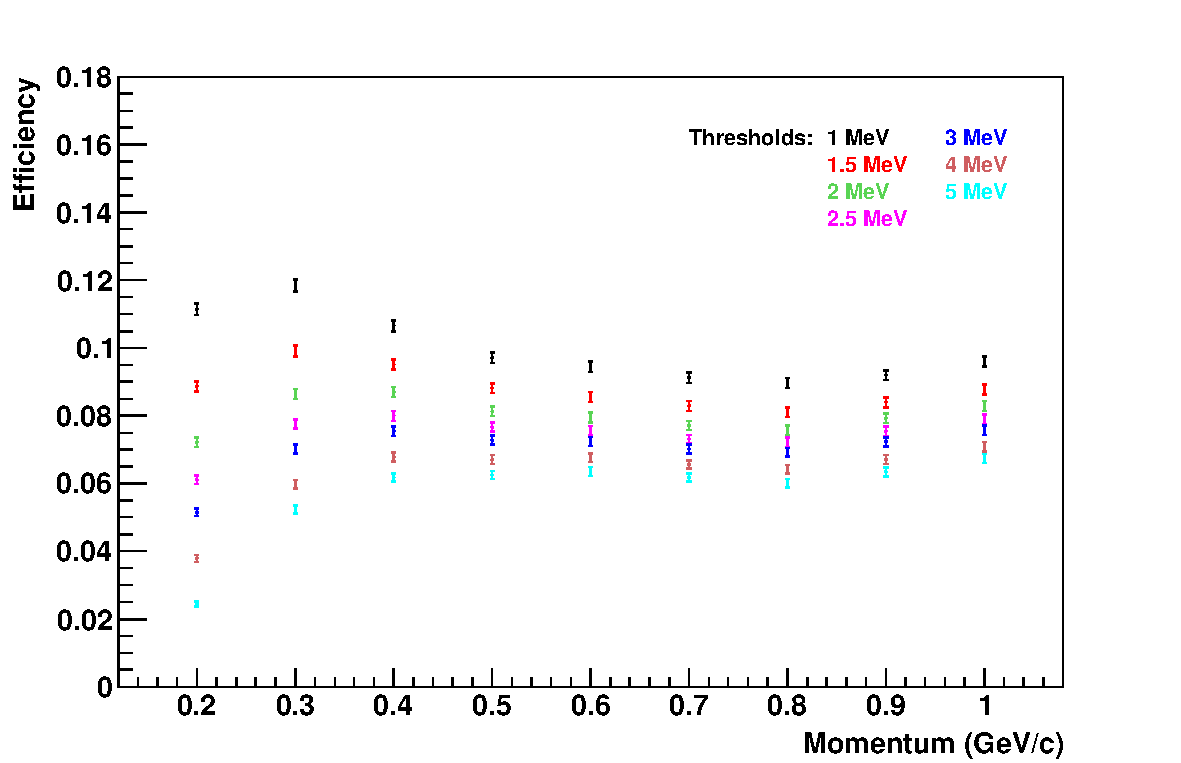
\includegraphics[width=0.5\textwidth]{Figure/eff_vs_mom_diff_thresh_II.pdf}
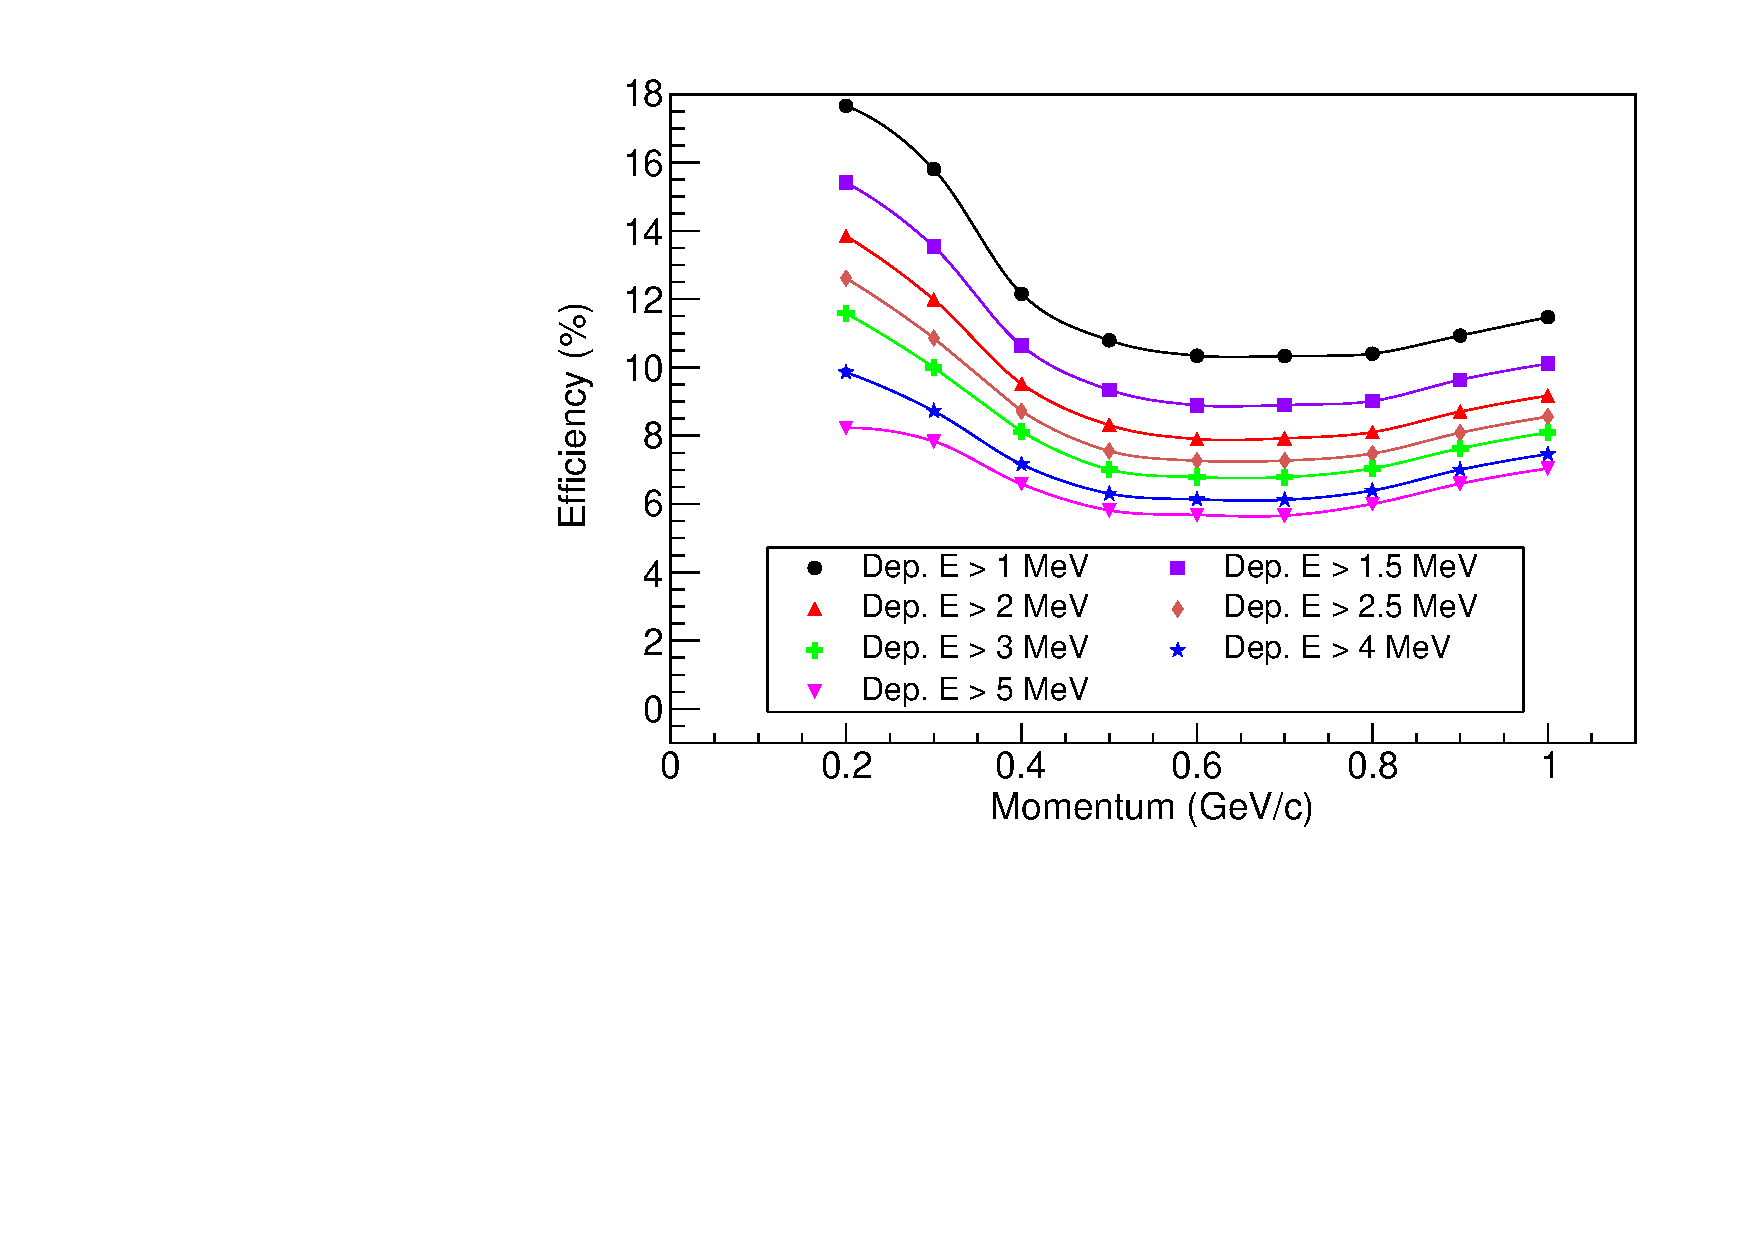
\includegraphics[width=0.45\textwidth]{Figure/Figure37.pdf}
\caption {Simulation results for the efficiency for the detection of neutrons emitted at $60^o$ as a function of momentum for 7 different values of the threshold on the deposited energy, from 1 to 5 MeV.}
\label{eff_vs_thr_mom}
\end{center}
\end{figure}
Figure~\ref{eff_vs_thr_mom} shows the neutron detection efficiency, which decreases with increasing threshold and ranges between 12\% at the lowest thresholds and 7\% at the highest ones. 
The angular resolution $\sigma_\theta$, obtained via Gaussian fits of the simulated $\theta$ distributions, increases slightly with the angle and also is fairly constant as a function of neutron momentum with its values between $1.8^o$ and $3^o$. 
The resolution on the azimuthal angle is directly connected to the total number of scintillator bars along $\phi$. The angular size of each bar, $\Delta\phi$, being 7.5$^{\circ}$, %\begin{eqnarray} 
%\Delta\phi = \frac{360^{\circ}}{48}=7.5^{\circ}.
%\end{eqnarray}
%where $N_{paddle}$ is the ID number of the paddle where the hit took place, and $N$ is the total number of paddles in $\phi$ ($N=48$). 
$\sigma_\phi$ is given by $\Delta\phi/2=3.75^o$.
The resolution on the neutron momentum, which is obtained knowing $\beta$ and having performed the particle identification, according to the formula
\begin{eqnarray}
p = \frac{\beta\cdot m_n}{\sqrt{1-\beta^2}},
\end{eqnarray}
is also strictly connected to the time resolution. The momentum resolution $\sigma_p/p$ ranges between 4.5\% and 6\%, for increasing neutron momentum. No appreciable variation of momentum resolution was observed by varying the neutron polar angle. As for the $\theta$ reconstruction, also in this case the reconstructed momentum was computed as the average over all layers, whenever more than one layer had a good hit.

Since the charged particles passing through the CND will be vetoed by the CVT, the only particles that could be mistaken for neutrons in the CND are photons. The efficiency of the CND for photons has been estimated by simulations, and it is slightly larger than for neutrons (of the order of 15\%, having little energy dependence). 
Neutrons can be discriminated from photons by means of their $\beta$.
%\begin{figure}[htb]  
%\begin{center}
%\includegraphics[width=0.45\textwidth]{Figure/Figure41.pdf}
%\caption {Efficiency for the detection of photons, as a function of photon momentum, for a 3-MeV threshold on the deposited energy. The efficiency is shown for $\theta_{\gamma}=60^o$. }
%\label{eff_photons}
%\end{center}
%\end{figure}
Therefore, the $\beta$ distributions that can be obtained with the CND for neutrons and photons were studied with the help of the GEMC simulation.
After choosing a good hit, $\beta$ is computed as  %as described in Appendix~\ref{sec_rec}, $\beta$ is computed as 
%
\begin{eqnarray}\label{beta_def}
\beta = \frac{l}{TOF_{true}\cdot c},
\end{eqnarray}
%
where 
\begin{eqnarray}\label{l_def} 
l = \sqrt{h^{2}+z_{ave}^{2}}.
\end{eqnarray}
%
$h$ is the distance from the vertex to the middle of the layer where the hit took place, $TOF_{true}$ is the reconstructed time-of-flight, and $z_{ave}$ is the reconstructed position of the hit along the scintillator bar. %(see Appendix~\ref{sec_rec} for more details on how the latter two quantities are obtained for the ``u-turn'' design of the CND)
%
Figure~\ref{beta_n_g} shows the comparison between the $\beta$ distributions obtained for neutrons of various momenta (0.2, 0.4, 0.7, and 1~GeV) and for 1-GeV photons. All particles in this plot were emitted at $\theta = 60^o$.
A small portion of the neutrons having momentum of 1~GeV can be taken as photons, as their $\beta$ distributions begin to overlap, while the $n/\gamma$ separation is clear for lower momenta --- which corresponds to most of the range of interest for $n$-DVCS, as only about 8\% of the events are expected to have $p_n>0.9$ GeV.
%
\begin{figure}[htb]  
\begin{center}
%\includegraphics[width=0.5\textwidth]{Figure/beta_comp_layer_1_II.pdf}
%\includegraphics[width=0.5\textwidth]{Figure/beta_comp_layer_2_II.pdf}
%\includegraphics[width=0.5\textwidth]{Figure/beta_comp_layer_3_II.pdf}
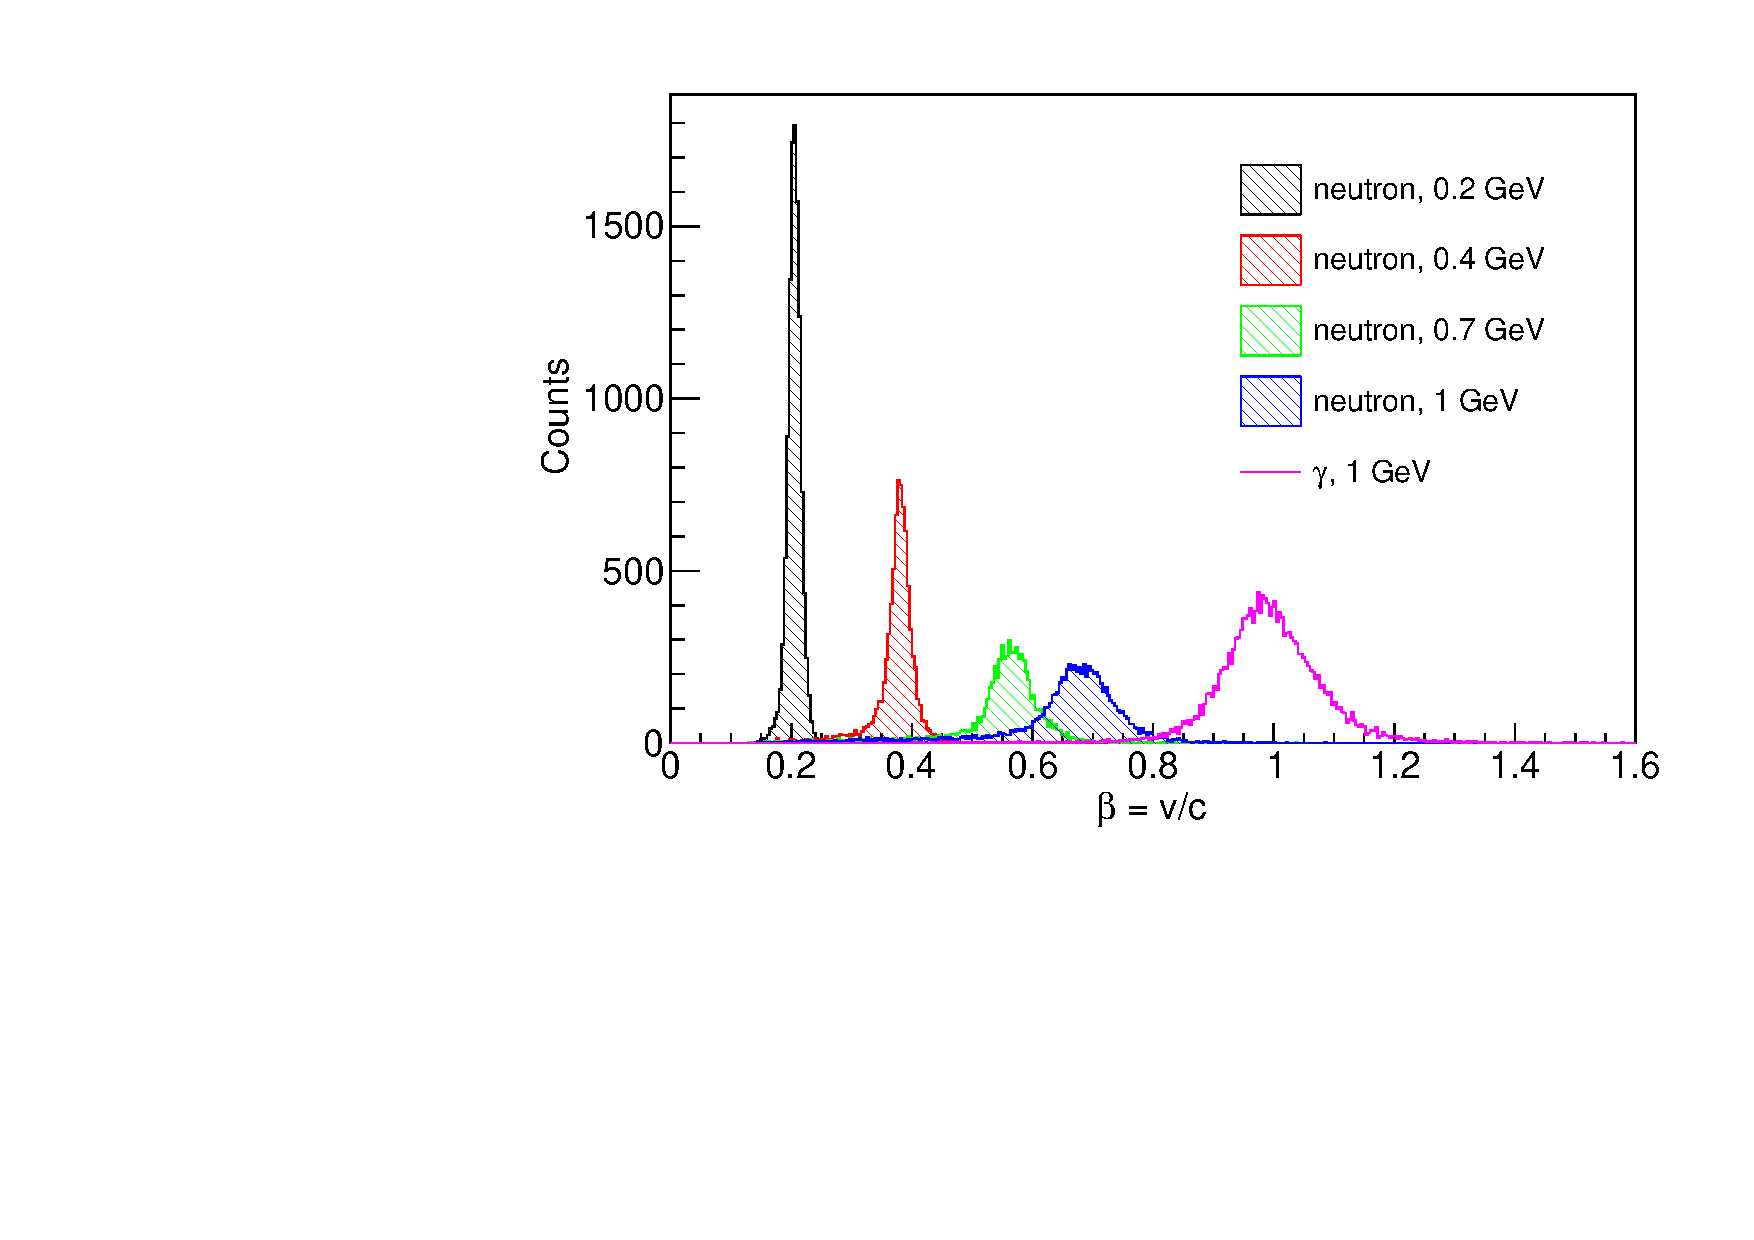
\includegraphics[width=0.45\textwidth]{Figure/Figure42.pdf}
\caption {Simulation results for the $\beta$ distributions for neutrons with $p_n=0.2$ GeV (black), $p_n=0.4$ GeV (red), $p_n=0.7$ GeV (green), $p_n=1$ GeV (blue), and photons with $E=1$ GeV (purple). The threshold on the deposited energy is 3 MeV. The plot show all reconstructed particles integrated over $\phi$. Equal neutron and photon yields were assumed.}
\label{beta_n_g}
\end{center}
\end{figure}

%\subsection{CND-based veto of charged particles}
%Section to be developed.
